\documentclass[t, screen, aspectratio=43]{beamer}
\usepackage[T1]{fontenc}
\usepackage[utf8]{inputenc}
\usepackage{epsf}
\usepackage{graphicx}
\usepackage{geometry}
\usepackage{tabularx}
\usepackage[table]{colortbl}
\usepackage{xcolor}
\usepackage{soul}
\usepackage[normalem]{ulem}
\usepackage{tikz}
\usepackage{subcaption}
% Use the NTNU-temaet for beamer 
% \usetheme[style=ntnu|simple|vertical|horizontal, 
%     language=bm|nn|en, 
%     smalltitle, 
%     city=all|trondheim|alesund|gjovik]{ntnu2017}
\usetheme[style=helvet,language=en]{ntnu2017}

\usepackage[english]{babel}
\usepackage[style=numeric,backend=biber,natbib=false,sorting=none]{biblatex}

\title[Short title]{Ultra low power integer-N ADPLL}
\subtitle{Master's thesis project - meeting 1}
\author[C Nielsen]{Cole Nielsen}
\institute[NTNU]{Department of Electronic Systems, NTNU}
\date{17 January 2020 (calendar week 3)}
%\date{} % To have an empty date

\addbibresource{example.bib} % Add bibliography database

% Set the reference style to numeric.
% See here: http://tex.stackexchange.com/questions/68080/beamer-bibliography-icon
\setbeamertemplate{bibliography item}[text] 

% Set bibliography fonts to a small size.
\renewcommand*{\bibfont}{\footnotesize}




\begin{document}

\begin{frame}
	\titlepage%
\end{frame}

% Alternatively, special title page command to get a different background
% \ntnutitlepage

% #############################################################################
% This week
% #############################################################################

\begin{frame}
	\frametitle{Timeline Tasks}
	\begin{block}{Project description}
		\begin{itemize}
			\footnotesize
			\item An ultra low power phase locked loop (PLL) frequency synthesizer shall be developed in 22nm FDSOI technology for application to 2.4 GHz ISM band wake up radio receivers. The project shall be undertaken with the following activities:
			\begin{itemize}
				\footnotesize
				\item Identification of an appropriate PLL architecture for ultra-low power consumption.
				\item Modeling of PLL to develop satisfactory specifications for PLL components.
				\item Transistor level implementation of design, including layout.
				\item Yield improvement/optimization if time allows.
			\end{itemize} 
		\end{itemize}    
	\end{block}
\end{frame}


% #############################################################################
% Timeline
% #############################################################################

\begin{frame}
	\frametitle{Time plan}
	\begin{block}{High level breakdown}
		\begin{itemize}
			\footnotesize
			\item \textbf{Modeling/test bench creation} (2 weeks)
			\begin{itemize}
				\footnotesize
				\item Finish high level modeling in Python to establish final component-level specifications.
				\item Finish ideal PLL model in Virtuoso (Verilog modeling?), create set of test benches.
			\end{itemize} 
			\item \textbf{Schematic/RTL design} (8 weeks)
			\begin{itemize}
				\footnotesize
				\item Schematic design for phase detector, oscillator, divider, calibration circuits
				\item RTL/synthesis/place\&route for digital loop filter and calibration circuits.
			\end{itemize} 
			\item \textbf{Layout} (4 weeks)
			\begin{itemize}
				\footnotesize
				\item Layout for phase detector, oscillator divider, calibration circuits.
			\end{itemize} 
		\item \textbf{Flex weeks} (2 weeks)
			\begin{itemize}
				\footnotesize
				\item One extra week for schematic design/layout respectively.
			\end{itemize} 
			\item \textbf{Report} (4 weeks)
		\end{itemize}    
	\end{block}
\end{frame}

\begin{frame}
	\frametitle{Time plan (pt. 1)}
	\begin{table}[htb!]
		\tiny
		\centering
		\vspace{-1em}
		\def\arraystretch{1.5}		
		\setlength\arrayrulewidth{0.75pt}
		\setlength{\tabcolsep}{1em} % for the horizontal padding
		\begin{tabular}{|l|l|l|l|}
			\hline 
			\rule[-1ex]{0pt}{2.5ex} \cellcolor{gray!40}\textbf{Week \#} & \cellcolor{gray!40}\textbf{Dates} &\cellcolor{gray!40}\textbf{Tasks} & \cellcolor{gray!40}\textbf{Outcomes}\\ 
			\hline 
			% \rule[-1ex]{0pt}{2.5ex} \cellcolor{green!20}\textbf{3}&\cellcolor{green!20}13.1 - 19.1 &\cellcolor{green!20}Review PLL Design &\cellcolor{green!20}Refreshed Knowledge\\ 
			% \hline 
			\rule[-1ex]{0pt}{2.5ex} \textbf{4}& 20.1 - 26.1 & Finalize high level modeling & Component level specification\\ 
			\hline 
			\rule[-1ex]{0pt}{2.5ex} \textbf{5}& 27.1 - 2.2 & Establish test bench in Virtuoso & With ideal PLL implementation\\ 
			\hline 
			\rule[-1ex]{0pt}{2.5ex} \textbf{6}& 3.2 - 9.2& Schem. design: phase detector & TDC - flash and counter based \\ 
			\hline 
			\rule[-1ex]{0pt}{2.5ex} \textbf{7}& 10.2 - 16.2& Schem. design: phase detector & Bang-bang phase detector\\ 
			\hline 
			\rule[-1ex]{0pt}{2.5ex} \textbf{8}&17.2 - 23.2& RTL, synthesis, place\&route & Digital loop filter\\ 
			\hline 
			\rule[-1ex]{0pt}{2.5ex} \textbf{9}&24.2 - 1.3& RTL, synthesis, place\&route & Digital loop filter\\ 
			\hline 
			\rule[-1ex]{0pt}{2.5ex} \textbf{10}&2.3 - 8.3& Schem. design: oscillator & Ring DCO\\ 
			\hline 
			\rule[-1ex]{0pt}{2.5ex} \textbf{11}&9.3 - 15.3& Schem. design: oscillator & LC DCO\\ 
			\hline 
			\rule[-1ex]{0pt}{2.5ex} \textbf{12}&16.3 - 22.3& Schem. design: divider  &TSPC + pulse swallow or sync counter?\\ 
			\hline 
			\rule[-1ex]{0pt}{2.5ex} \textbf{13}&23.3 - 29.3&Schem. design: Calibration& RTL/schem. for calibration\\ 
			\hline 
			\rule[-1ex]{0pt}{2.5ex} \textbf{14}& 30.3 - 5.4 &  Flex week - schem. design & Finalize schematic level design\\ 
			\hline 
			\rule[-1ex]{0pt}{2.5ex} \textbf{15}& 6.4 - 12.4& {\color{red}\textbf{Easter}} & - \\ 
			\hline 
			\rule[-1ex]{0pt}{2.5ex} \textbf{16}& 13.4 - 19.4& Layout & Phase detector\\ 
			\hline 
			\rule[-1ex]{0pt}{2.5ex} \textbf{17}& 20.4 - 26.4& Layout & Oscillator\\ 
			\hline 
		\end{tabular}
		\begin{flushleft}\textbf{Legend:} \colorbox{red!20}{\textbf{Done}} \colorbox{green!20}{\textbf{Current}}  \colorbox{blue!20}{\textbf{Revised}}
		% *I will write the report simultaneously with the work.
		\end{flushleft}
		% \caption{Assigned specifications for branch line hybrid design.}
		% \label{asgn_specs}
	\end{table}   
\end{frame}

\begin{frame}
	\frametitle{Time plan (pt. 2)}
	\begin{table}[htb!]
		\tiny
		\centering
		\vspace{-1em}
		\def\arraystretch{1.5}		
		\setlength\arrayrulewidth{0.75pt}
		\setlength{\tabcolsep}{1em} % for the horizontal padding
		\begin{tabular}{|l|l|l|l|}
			\hline 
			\rule[-1ex]{0pt}{2.5ex} \cellcolor{gray!40}\textbf{Week \#} & \cellcolor{gray!40}\textbf{Dates} &\cellcolor{gray!40}\textbf{Tasks} & \cellcolor{gray!40}\textbf{Outcomes}\\ 
			\hline 
			\rule[-1ex]{0pt}{2.5ex} \textbf{18}& 27.4 - 3.5 & Layout & Divider/calibration\\ 
			\hline 
			\rule[-1ex]{0pt}{2.5ex} \textbf{19}& 4.5 - 10.5 & Layout & Finalization/system integration\\ 
			\hline 
			\rule[-1ex]{0pt}{2.5ex} \textbf{20}& 11.5 - 17.5 & Flex week (layout) OR yield improvement & Depending on progress\\ 
			\hline 
			\rule[-1ex]{0pt}{2.5ex} \textbf{21}& 18.5 - 24.5& {\color{blue}\textbf{Report writing}} & \\ 
			\hline 
			\rule[-1ex]{0pt}{2.5ex} \textbf{22}& 25.5 - 31.5& {\color{blue}\textbf{Report writing}} & \\ 
			\hline 
			\rule[-1ex]{0pt}{2.5ex} \textbf{23}& 1.6 - 7.6& {\color{blue}\textbf{Report writing}} & {\color{red}\textbf{Deadline 8.6}}\\ 
			\hline 
		\end{tabular}
		\begin{flushleft}\textbf{Legend:} \colorbox{red!20}{\textbf{Done}} \colorbox{green!20}{\textbf{Current}}  \colorbox{blue!20}{\textbf{Revised}}
		% *I will write the report simultaneously with the work.
		\end{flushleft}
		% \caption{Assigned specifications for branch line hybrid design.}
		% \label{asgn_specs}
	\end{table}   
\end{frame}




% #############################################################################
% This week
% #############################################################################






% #############################################################################
% Loop Dynamics (continuous)
% #############################################################################

% \begin{frame}
% 	\frametitle{Loop Dynamics}
% 	\begin{block}{Still To Do}
% 		\vspace{-.2em}
% 		\begin{itemize}
% 			\footnotesize
% 			\item Standard approach to used mixed continuous/discrete time mathematical model for DPLL. 
% 			\item Plot of RO phase noise (typical)
% 			\item Automatic analysis of performance (lock detection, residual phase modulation, lock-in/pull-in range).
% 			\item Automatic optimization (using gradient descent) of PLL parameters?
% 			\item Z-domain modeling of loop? Develop (by hand) some ideal transfer funtions for loop.

% 		\end{itemize}    
% 	\end{block}
% \end{frame}

% #############################################################################
% Architecture - block diagram
% #############################################################################

\begin{frame}
	\frametitle{State of the Art}
	\begin{block}{Sub 1-mW PLLS}
		\footnotesize Application is niche, so comparable PLLs hard to find. Sub 100$\mu$W is a reasonable target for low-power state of art in 2.4 GHz PLLs.
		\vspace{-1em}
		\begin{table}[htb!]
			\tiny
			\centering
			\def\arraystretch{1.5}		
			\setlength\arrayrulewidth{0.75pt}
			\setlength{\tabcolsep}{1em} % for the horizontal padding
			\begin{tabular}{|l|l|l|l|l|l|l|l|}
				\hline 
				\rule[-1ex]{0pt}{2.5ex} \cellcolor{gray!40}\textbf{Type} & \cellcolor{gray!40}\textbf{P$_{PLL}$ [$\mu$W]}& \cellcolor{gray!40}\textbf{P$_{osc}$ [$\mu$W] }& \cellcolor{gray!40}\textbf{Freq [MHz]} & \cellcolor{gray!40}\textbf{PN@$\Delta f$ [dBc/Hz]}& \cellcolor{gray!40}\textbf{t$_{lock}$* [$\mu$s]}& \cellcolor{gray!40}\textbf{Osc. }& \cellcolor{gray!40}\textbf{Ref Freq}\\ 
				\hline 
				\rule[-1ex]{0pt}{2.5ex} \textbf{Dig. Frac-N} & 650 & 304 & 2400 & -110@0.5M & 15/4 & LC & 26M\\ 
				\hline 
				\rule[-1ex]{0pt}{2.5ex} \textbf{Ana. Int-N }& 680 & 510 & 2400 & -110@1M & 130/70 & LC & 1M\\ 
				\hline 
				\rule[-1ex]{0pt}{2.5ex} \textbf{Ana. Int-N} & 128 &  & 500 & -94@1M &  & Ring & 31.25M\\ 
				\hline 
				\rule[-1ex]{0pt}{2.5ex} \textbf{Ana. Int-N} & 570 &  & 800 & -92.6@0.1M & 200 & LC & 0.2M\\ 
				\hline 
				\rule[-1ex]{0pt}{2.5ex} \textbf{Dig. Frac-N} & 250 & 173 & 2448 &  & 22/1 & Ring & 9M\\ 
				\hline 
				\rule[-1ex]{0pt}{2.5ex} \textbf{Ana. Int-N} & 950 &  & 5500 & -106@1M &  & IL-LC & \\ 
				\hline 
			\end{tabular} 
			% \caption{Assigned specifications for branch line hybrid design.}
			% \label{asgn_specs}
		\end{table}  

	\end{block}

\end{frame}

\begin{frame}
	\frametitle{Architecture}
	\begin{block}{Block Diagram}
	\center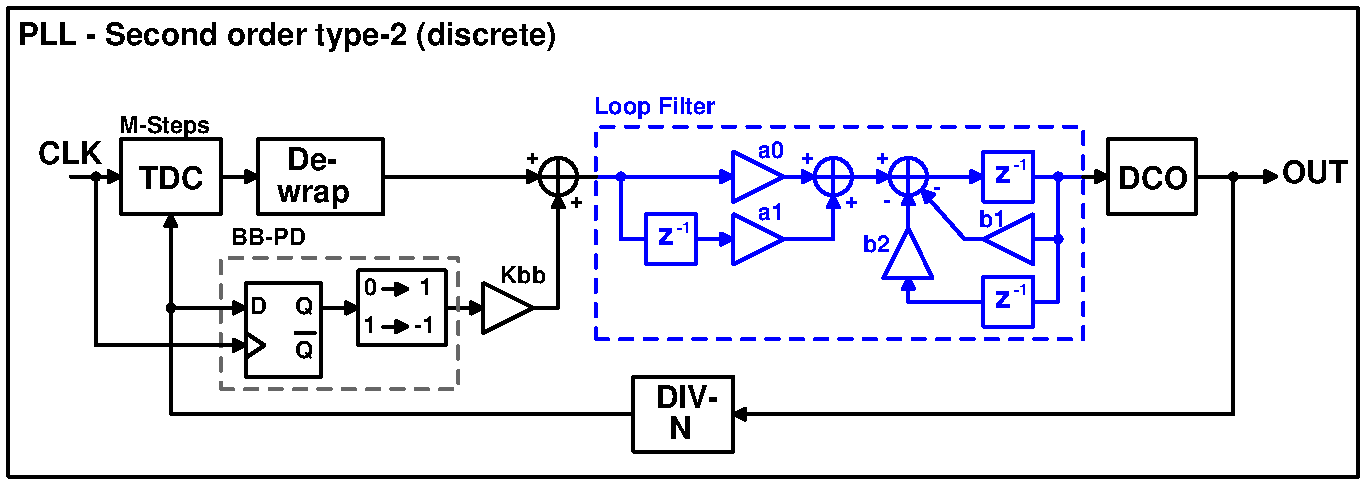
\includegraphics[width=0.8\textwidth, angle=0]{pll_sec_order_bb.pdf}

	\end{block}
		\begin{block}{Power Targets}
		\vspace{-.1em}
		\begin{table}[htb!]
			\tiny
			\centering
			\def\arraystretch{1.5}		
			\setlength\arrayrulewidth{0.75pt}
			\setlength{\tabcolsep}{1em} % for the horizontal padding
			\begin{tabular}{|l|l|l|l|l|l|}
				\hline 
				\rule[-1ex]{0pt}{2.5ex} \cellcolor{gray!40}\textbf{DCO} & \cellcolor{gray!40}\textbf{Phase detector} & \cellcolor{gray!40}\textbf{Divider }& \cellcolor{gray!40}\textbf{Digital (LF)}& \cellcolor{gray!40}\textbf{Other} & \cellcolor{gray!40}\textbf{SUM} \\ 
				\hline 
				\rule[-1ex]{0pt}{2.5ex} 50 $\mu$W& 10 $\mu$W & 10 $\mu$W & 10 $\mu$W  & $<<$ 10 $\mu$W & $<$ 100 $\mu$W\\ 
				\hline 
			\end{tabular} 
			% \caption{Assigned specifications for branch line hybrid design.}
			% \label{asgn_specs}
		\end{table}   
	\end{block}

\end{frame}

% #############################################################################
% Specification
% #############################################################################

\begin{frame}
	\frametitle{Specification\color{black}}
	\begin{block}{System Performance Targets}
		\scriptsize
		\begin{table}[h!]
			\centering
			\def\arraystretch{1.5}		
			\setlength\arrayrulewidth{0.75pt}
			\setlength{\tabcolsep}{1em} % for the horizontal padding
			\begin{tabular}{|l|r|l|l|}
				\hline 
				\rule[-1ex]{0pt}{2.5ex} \cellcolor{gray!40}\textbf{Parameter} & \cellcolor{gray!40}\textbf{Value} & \cellcolor{gray!40}\textbf{Unit }& \cellcolor{gray!40}\textbf{Notes}\\ 
				\hline 
				\rule[-1ex]{0pt}{2.5ex} \textbf{Frequency}  & 2.4-2.4835 & GHz & 2.4G ISM Band\\ 
				\hline 
				\rule[-1ex]{0pt}{2.5ex} \textbf{Ref. frequency} & 16 & MHz & Yields 6 channels \\ 
				\hline 
				\rule[-1ex]{0pt}{2.5ex} \textbf{Power} & $\leq$ 100  &$\mu$W & minimize!\\ 
				\hline 
				\rule[-1ex]{0pt}{2.5ex} \textbf{FSK BER} & $\leq$ 1e-2  & & 2FSK with $f_{dev}$=$\pm$250 KHz\\ 
				\hline 
				\rule[-1ex]{0pt}{2.5ex} \textbf{Initial Lock Time} & $\leq$ 10 & $\mu$s & Upon cold start \\ 
				\hline 
				\rule[-1ex]{0pt}{2.5ex} \textbf{Re-lock Time} & $\leq$ 5 & $\mu$s & Coming out of standby \\ 
				\hline 
			\end{tabular} 
			% \caption{Assigned specifications for branch line hybrid design.}
			% \label{asgn_specs}
		\end{table}   
		Additionally: PLL output should support IQ sampling at LO frequency.
	\end{block}    
\end{frame}



% #############################################################################
% project phases
% #############################################################################

% ############################################################################b#
% References
% #############################################################################


% \begin{frame}
% 	\frametitle{References}
% 		\scriptsize
% 		[1] "Ultra-Low Power Wake-Up Receivers for Wireless Sensor Networks", N. Pletcher, J.M Rabaey, 2008.\\
% 		\hspace{16pt}\url{http://www.eecs.berkeley.edu/Pubs/TechRpts/2008/EECS-2008-59.html}\\
% 		\vspace{1em}
% 		% [2] "Minimum Achievable Phase Noise of RC Oscillators",
% 	% Navid et al. 2005
% \end{frame}


\end{document}
